\section{Initial Search Criteria}
The primary objective of the analysis discussed in this dissertation is to search for electroweak supersymmetry with tri-leptonic signatures and large missing transverse energy, $E_{T}^{miss}$. 
This tri-leptonic decay signature comes from the SM decay of a $W$ boson and, specifically, a leptonic decay of a $Z$ boson. This particular interaction can be represented below.

\begin{figure}[H] %  figure placement: here, top, bottom, or page
   \centering
   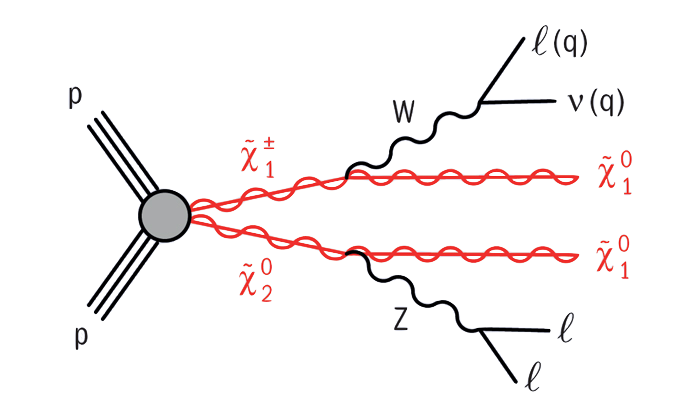
\includegraphics[width=0.7\textwidth]{Pictures/WZSUSY.png} 
   \caption{$WZ$ mediated SUSY production from $pp$ collision resulting in tri-leptonic final state}
   \label{fig:SUSYWZ}
\end{figure}

\noindent What we see here is, in the upper portion of the diagram, the lightest chargino mass eigenstate decaying to a $W$ boson and an LSP. 
This is then followed by $W$ boson decay to one lepton and a neutrino.

\begin{align}
\tilde{\chi}_{1}^{\pm} &\rightarrow W + \tilde{\chi}_{1}^{0} \\
W &\rightarrow \ell + \nu
\end{align}

\noindent In the lower portion of the diagram we have a neutralino in the second mass eigenstate decaying to an LSP and a $Z$ boson. This $Z$ boson then decays into a lepton anti-lepton pair.

\begin{align}
\tilde{\chi}_{2}^{0} &\rightarrow Z + \tilde{\chi}_{1}^{0} \label{eqn:ChiToZ} \\
Z &\rightarrow \ell + \bar{\ell}
\end{align}

\noindent In order to search for appropriate signatures that imply this interaction, stringencies must be placed on ones selection criteria. 
This is done such that uninteresting signatures - those occurring from SM interactions - can be attenuated.
Unfortunately not all of the uninteresting signatures can be attenuated and so one still maintains a SM background.

\subsection{Leptonic Signature Selection}
From consideration of the event diagram, shown in figure \ref{fig:SUSYWZ}, one can immediately suggest two features to include in event selection.
The obvious initial requirement is to detect a tri-leptonic signature seeing as this interaction results in three final state leptons.
The more subtle selection criteria comes in the lepton flavour choices.
We can write the $WZ$ decay as follows:

\begin{align}
WZ \rightarrow \left(Z \rightarrow \ell^{\pm} \ell^{\mp} \right) \left(W^{\pm} \rightarrow \ell^{\prime \pm}\right)
\end{align}

\noindent Naturally the leptons created as a result of $Z$ boson decay must be of the same flavour and have opposite electric charge.
Seeing as one obtains highly energetic leptons from $Z$ boson decay, compared to that from $W$ boson decay, these leptons become the leading and next to leading leptons. 
From this one can make a requirement that the leading and next to leading lepton pair must be a `same flavour opposite sign', SFOS, pair.

This requirement does not completely specify $WZ$ mediated SUSY production, however, as SFOS signatures can be obtained from $Wh$ mediated SUSY.
This is not entirely problematic as $Wh$ mediation can result in the Higgs particle decaying into a `different flavour opposite sign', DFOS, lepton pair; something the $Z$ boson can not without violating electron and muon number conservation.

\subsection{Event Selection Triggers}

\subsection{Veto of Bottom Quark Jets}
A particular cleaning cut is placed when going through the event selection.
This is to remove any signals that have hadronic jets initiated by bottom quarks.
This is an important tool as it substantially reduces the background events caused by top quarks; a well known Standard Model event.

Supposing a $t \bar{t}$ pair is created, the decay mode of this state is shown in figure \ref{fig:ttbar} below.

\begin{figure}[H] %  figure placement: here, top, bottom, or page
   \centering
   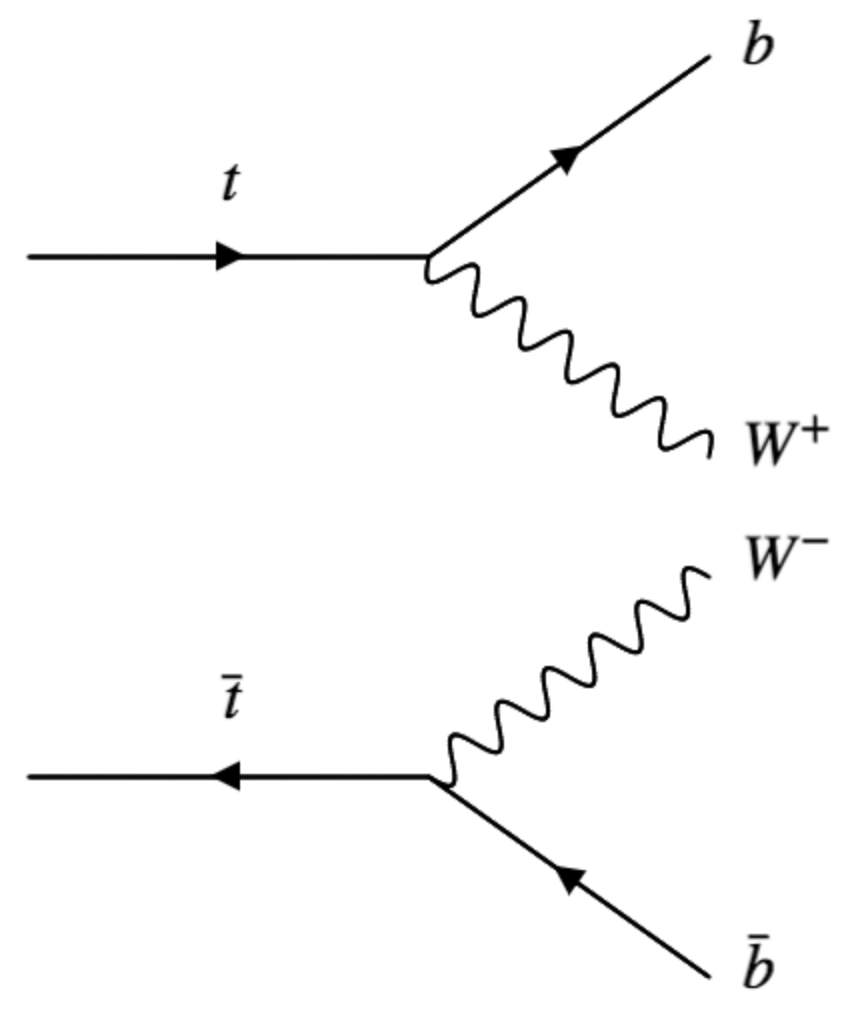
\includegraphics[width=0.4\textwidth]{Pictures/ttbar.png} a
   \caption{$t \bar{t}$ pair decaying to $b \bar{b}$ and two $W$ bosons}
   \label{fig:ttbar}
\end{figure}

\noindent In either the $t$ or the $\bar{t}$ scenarios, the resultant bottom quark, or anti-quark, will thusly initiate a hadronic jet, referred to as b-jets.
Fortuitously, $b$-jets have certain features making it possible to identify them from other flavour jets.  
As a result of this b-jet tagging, one is able to specify whether or not to include them in the search criteria.
Seeing as we are not looking for hadronic final states from the SUSY interaction, the search criteria ignores all tagged $b$-jets signals.
\textbf{\large discuss b-tagging}

\subsection{Mass Shells} \label{subsec:MassShells}
Within the neutral portion of the SUSY interaction, given in equation \ref{eqn:ChiToZ}, there is the potential to produce an on shell $Z$ boson, or an off shell virtual $Z$ boson.
Whether the mediating boson is on or off shell means the lepton pair produced may have very different invariant masses.

\begin{figure}[H] %  figure placement: here, top, bottom, or page
   \centering
   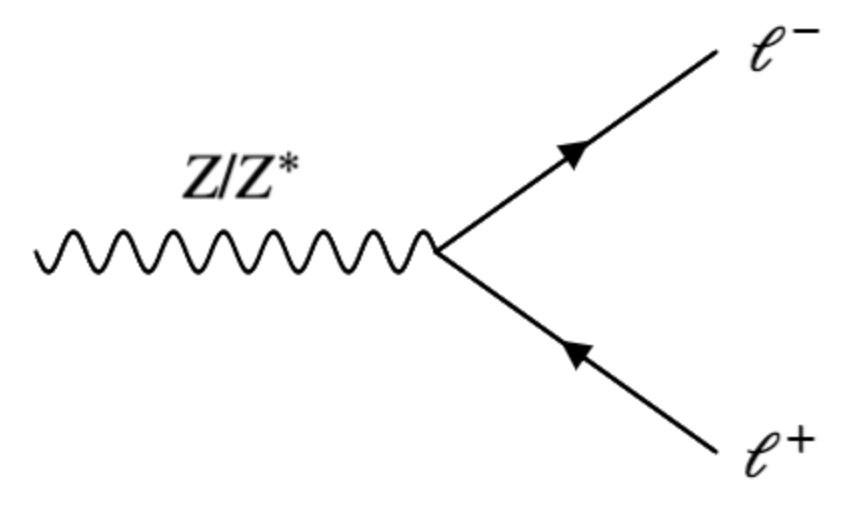
\includegraphics[width=0.5\textwidth]{Pictures/ZtoLL.png} 
   \caption{Real or virtual $Z$ boson decay to a same flavour, opposite sign lepton pair}
   \label{fig:example}
\end{figure}

\noindent From the on shell lepton pair one should be able to reconstruct the mass of the real $Z$ boson, however, virtual $Z$ bosons will result in the reconstruction of a mass significantly above or below the true value.
This is not an issue as it allows for a splitting in analysis procedure. 
One can thereby examine on shell and off shell events separately.

Below shows the invariant mass distribution of the two leptons associated with the $Z$ boson.

\begin{figure}[H] %  figure placement: here, top, bottom, or page
   \centering
   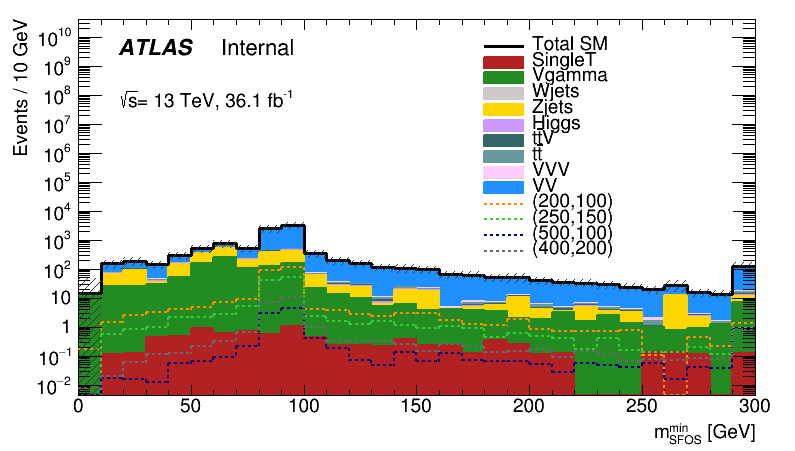
\includegraphics[width=0.7\textwidth]{Pictures/ZmassDist.png} 
   \caption{Invariant mass distribution of same flavour, opposite sign lepton pair}
   \label{fig:L1L2InvariantMass}
\end{figure}

\noindent The solid coloured blocks capped with the thick black line are the Standard Model backgrounds, discussed in \textbf{\large BACKGROUNDS SECTION}.
The dashed lines are the simulated SUSY samples generated using Monte Carlo techniques.
We can see clearly that there exists a peak in the distribution of both the backgrounds and the samples centred at roughly $90$ GeV, spanning from $80 - 100$ GeV.
This is clearly a $Z$ mass peak and so we can divide analyses accordingly.
Luckily, the mass of the $Z$ boson is a well known quantity and so we are able to define mass shell regions with a high degree of specificity.
The agreed requirements for the on and off shell analyses are thereby defined as:

\begin{align} 
\textrm{On Shell:}\ \ m_{\textrm{SFOS}}^{min} \in [81.2, 101.2] \\
\textrm{Off Shell:}\ \ m_{\textrm{SFOS}}^{min} \notin [81.2, 101.2].
\end{align}



\begin{figure}[H]
    \centering
    \begin{subfigure}[b]{0.48\textwidth}
        \centering
        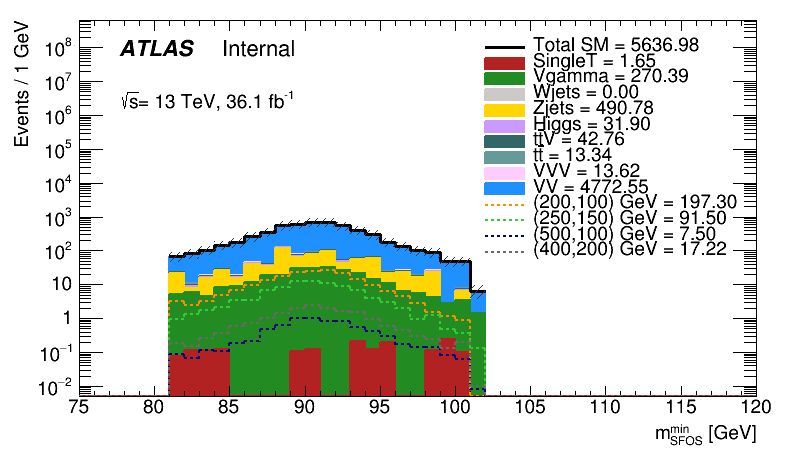
\includegraphics[width=\textwidth]{Pictures/OnMassShell.png}
    \caption{}
    \end{subfigure}
    ~
    \begin{subfigure}[b]{0.48\textwidth}
        \centering
        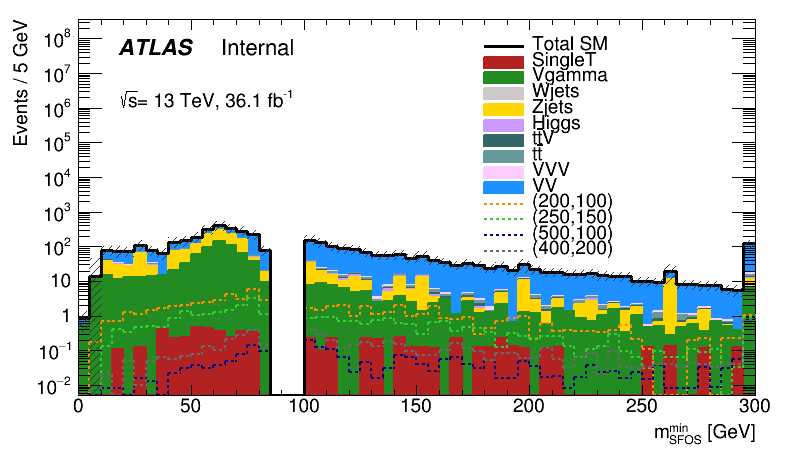
\includegraphics[width=\textwidth]{Pictures/OffMassShell.png}
    \caption{}    
        \end{subfigure}
\caption{(a) On shell invariant mass distribution of same flavour, opposite sign lepton pair.
(b) Off shell invariant mass distribution of same flavour, opposite sign lepton pair.}
\label{fig:ATLAS}
\end{figure}

\subsection{This is a table}

\begin{center}
\begin{tabular}{c c c c c c}
\toprule
Sample& 3$\ell$& + SFOS& + b-jet veto& + onZ\\

\midrule
ttV& $ 425.65 \pm 1.29 $& $ 401.57 \pm 1.25 $& $ 64.20 \pm 0.55 $& $ 42.76 \pm 0.46 $\\
single top& 	 $18.4\pm 1.46$& 	 $14.13\pm 1.29$& 	 $8.32\pm 0.99$& 	 $1.65\pm 0.43$\\
$Z$+jets Sherpa& 	 $1471.08\pm 120.23$& 	 $1467.4\pm 120.16$& 	 $1365.1\pm 118.73$& 	 $490.78\pm 62.66$\\
$W$+jets& 	 $0.23\pm 0.15$& 	 $0.08\pm 0.07$& 	 $0.08\pm 0.07$& 	 $0.0\pm 0.0$\\
VV& 	 $7455.16\pm 17.85$& 	 $7393.23\pm 17.8$& 	 $7149.44\pm 17.68$& 	 $4772.79\pm 14.91$\\
ttbar& 	 $299.83\pm 4.5$& 	 $223.78\pm 3.9$& 	 $74.67\pm 2.26$& 	 $13.34\pm 0.95$\\
Vgamma& 	 $1059.41\pm 17.91$& 	 $1055.8\pm 17.89$& 	 $1027.89\pm 17.66$& 	 $270.39\pm 8.88$\\
Higgs& 	 $81.88\pm 4.83$& 	 $73.05\pm 4.54$& 	 $61.78\pm 4.43$& 	 $31.9\pm 3.0$\\
Tribosons& 	 $54.95\pm 0.67$& 	 $45.52\pm 0.6$& 	 $43.87\pm 0.59$& 	 $13.62\pm 0.28$\\
\hline
Total background& 	 $10866.58\pm123.05$& 	 $10674.57\pm122.94$& 	 $9795.36\pm121.44$& 	 $5637.22\pm65.1$\\
\hline\hline
via WZ (200,100)& 	 $267.35\pm 4.51$& 	 $266.9\pm 4.51$& 	 $261.59\pm 4.46$& 	 $197.3\pm 3.87$\\
via WZ (250,150)& 	 $124.57\pm 2.02$& 	 $124.4\pm 2.02$& 	 $121.81\pm 2.0$& 	 $91.5\pm 1.73$\\
via WZ (500,100)& 	 $10.79\pm 0.3$& 	 $10.73\pm 0.29$& 	 $10.4\pm 0.29$& 	 $7.5\pm 0.25$\\
via WZ (400,200)& 	 $23.88\pm 0.5$& 	 $23.84\pm 0.5$& 	 $23.34\pm 0.49$& 	 $17.22\pm 0.42$\\
\bottomrule
\end{tabular}
\end{center}

\section{Improving Event Selection with Variable Cuts}